\section{Detailed Explanation}
    In this part, we take a look at ``detailed explanation'' and try to figure it out which
    factors should be taken into consideration when we start to design a good detailed explanation.
    And an example is also provided in order to illustrating how these factors are used in industrial product nowadays.
    \subsection{Seven Explanatory Criterion}

        \indent 
        Like what we have already mentioned in the overview, the ``seven explanatory criterion''\cite{tintarev2007survey}(see table \ref{table:1}) from Nava Tintarev and Judith Masthoff
        is the most popular standard used to evaluate the explanation. 
        It is also comprehensive since it takes all aspects, which is relevant to design a good explanation, into consideration.
        Thus these seven explanatory criterion are useful if we want to design a detailed explanation.
        \begin{table}[ht] 
            % ht used to attach the table to the position approximately where they are wrote here
            \centering
            \begin{tabular}{ | m{8em} | m{4cm} | }
            \hline
            %  \bfseries used to bold the header
            \bfseries Aim & \bfseries Definition\\ [0.5ex] 
            \hline\hline
            Transparency & Explain how the system works\\ 
            \hline
            Scrutability & Allow users to tell the system it is wrong\\ 
            \hline
            Trust & Increase users' confidence in the system\\ 
            \hline
            Effectiveness & Help users make good decisions\\ 
            \hline
            Persuasiveness & Convince users to try\\ 
            \hline
            Efficiency & Help users make decisions faster\\ 
            \hline
            Satisfaction & Increase the ease of use or enjoyment\\ 
            \hline
            \end{tabular}
            \caption{Explanatory criteria and their definitions}
            \label{table:1}
        \end{table}

        \indent Although they may called differently in different research works
        (``explanation attributes''\cite{al2013explanations}, ``seven possible aims for explanations''\cite{tintarev2012evaluating}
        or ``quality factors''\cite{gedikli2014should}).
        The basic idea is the same, which aims at making system more understandable by users.
        
        \indent \textbf{\textit{Transparency:}} Transparency in a recommender system is related to
         the capability of a system to expose the reasoning behind a recommendation to its users\cite{herlocker2000explaining}.
         A recommender systems without explanation works like a ``black box'', which may lost trust from user. 
         Thus, transparency is considered as an important factor to build user's trust in the system\cite{swearingen2002interaction}.

        \indent \textbf{\textit{Scrutability:}} Scrutability means, in short, allow users to tell the system it is wrong.
        It can also be seen as a kind of User Control, which allows users to correct reasoning from system\cite{czarkowski2002scrutable}.
        
        \indent \textbf{\textit{Trust:}} Trust is sometimes linked with transparency.
        Studies have already shown that transparency and 
        the possibility of interaction with recommender systems increases user trust\cite{felfernig2007knowledge}\cite{sinha2002role}.
        
        \indent \textbf{\textit{Effectiveness:}} An effective explanation can help users to make a better decision.
        If an item suggested by the system is the one the user really likes, such explanation can be considered as effective.

        \indent \textbf{\textit{Persuasiveness:}} Persuasiveness, sometimes referred to as promotion, 
        is strongly related to effectiveness and 
        can be defined as the ability of an explanation type to convince the user to accept or disregard certain items\cite{gedikli2014should}.

        \indent \textbf{\textit{Efficiency:}} An explanation is usually considered to be efficient when
         it helps the user to decide more quickly or when it helps to reduce the cognitive effort required in the decision process\cite{gedikli2014should}.
         The most common approach to measure it is to look at the iteration time between users and recommender system before users reach their goals.

        \indent \textbf{\textit{Satisfaction:}} The user’s overall satisfaction with a recommender system is assumed to be 
        strongly related to the perceived quality of its recommendations and explanations\cite{swearingen2002interaction}.
 
    \subsection{Examples of Detailed Explanation}
        An example of explanation in amazon.com.
        TODO: (Write Analysis based on seven explanatory criterion) 
        \begin{figure}[H]
            \centering
            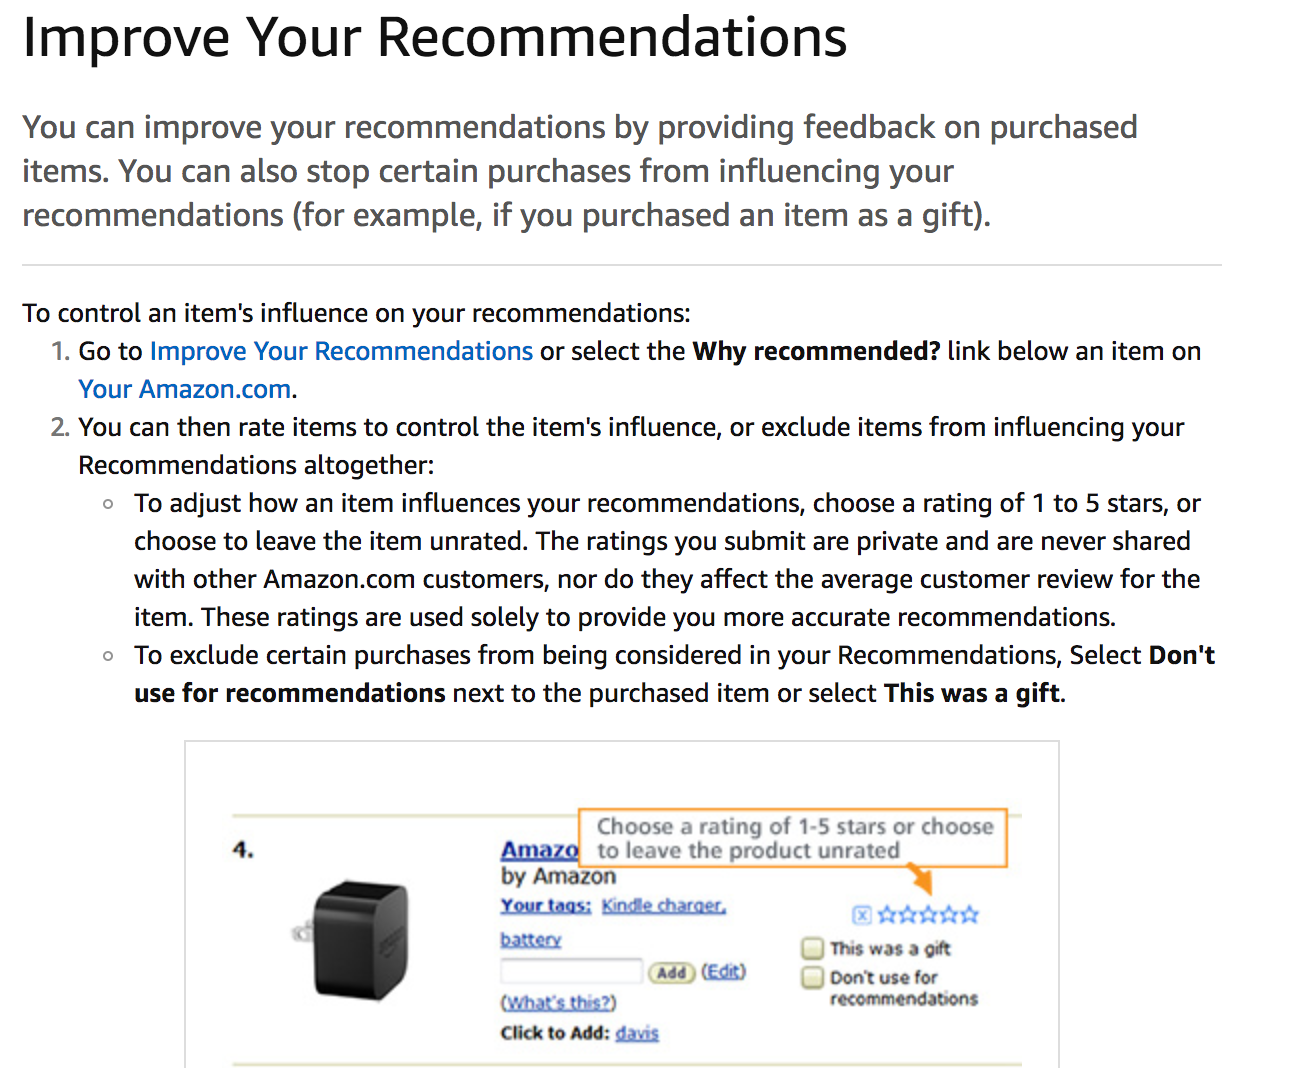
\includegraphics[width=0.5\textwidth]{img/amazon1}
            \caption{Amazon}
            \label{fig:amazon1}
        \end{figure}
        An example of explanation of Google Ads.
        TODO:  (Write Analysis based on seven explanatory criterion) 
        \begin{figure}[H]
            \centering
            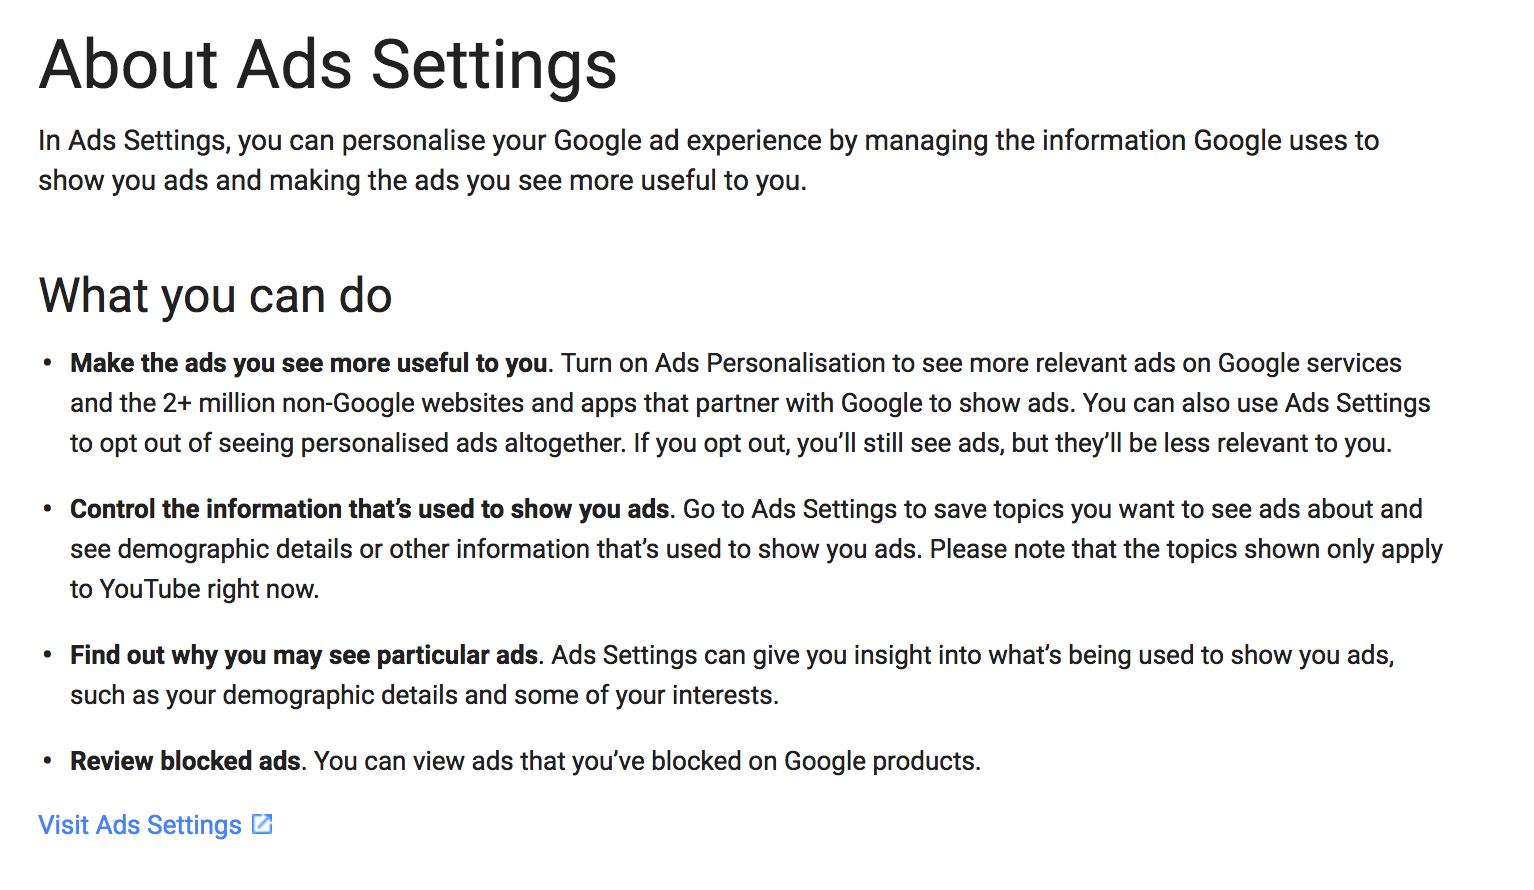
\includegraphics[width=0.5\textwidth]{img/google1}
            \caption{Google}
            \label{fig:google1}
        \end{figure}
\section{Short Explanation}
    However, in some scenario, a brief explanation is more suitable, for example, driving in a car
    (why: users have limited attention resource)
    We can not take all seven explanatory criterion into consideration.
    How to extract a kind of standards.
    
    \subsection{Possible Criterion for Short Explanation}

    \subsection{Examples of Short Explanation}
        Example1: Explanations in Proactive Recommender Systems in Automotive Scenarios \cite{bader122011explanations}
        \textbf{Extract two criterion out of seven explanatory criterion: Persuasiveness and Efficiency.}

        Example2: Why did my car just do that? Explaining semi-autonomous driving actions to improve driver understanding, trust, and performance\cite{koo2015did}
        \textbf{Extract two types (what and how)based on question types from Intelligent Toolkit} \cite{Brian2010toolkit, lim2011design}
